\documentclass{article}

% if you need to pass options to natbib, use, e.g.:
%     \PassOptionsToPackage{numbers, compress}{natbib}
% before loading neurips_2019

% ready for submission
% \usepackage{neurips_2019}

% to compile a preprint version, e.g., for submission to arXiv, add add the
% [preprint] option:
%     \usepackage[preprint]{neurips_2019}

% to compile a camera-ready version, add the [final] option, e.g.:
\usepackage[final]{neurips_2019}

% to avoid loading the natbib package, add option nonatbib:
%     \usepackage[nonatbib]{neurips_2019}

\usepackage[utf8]{inputenc} % allow utf-8 input
\usepackage[T1]{fontenc}    % use 8-bit T1 fonts
\usepackage{hyperref}       % hyperlinks
\usepackage{url}            % simple URL typesetting
\usepackage{booktabs}       % professional-quality tables
\usepackage{amsfonts}       % blackboard math symbols
\usepackage{nicefrac}       % compact symbols for 1/2, etc.
\usepackage{microtype}      % microtypography
\usepackage{amsmath}        % because
\usepackage{graphicx}       % pictures
\usepackage{xcolor}         % colored text

% Macros
\newcommand{\blue}[1]{\textcolor{blue}{#1}}

\title{}

% The \author macro works with any number of authors. There are two commands
% used to separate the names and addresses of multiple authors: \And and \AND.
%
% Using \And between authors leaves it to LaTeX to determine where to break the
% lines. Using \AND forces a line break at that point. So, if LaTeX puts 3 of 4
% authors names on the first line, and the last on the second line, try using
% \AND instead of \And before the third author name.

\author{%
  Mingcheng Wang, Eric Xia, Trevor Jung\\ % write a list of authors
  University of Washington \\
 \texttt{\{wmingch, ericxia, tjung2\}@uw.edu} \\ % write your email
}

\begin{document}

\maketitle
\bibliographystyle{unsrt}

% Template and style guide for the eproducibility project for CSE 517.

% Note that we slightly updated the style file for the CSE 517 project, so it is not exactly the same as 2020 ML Reproducibility Challenge (or later iterations).  In order to submit to a ML Reproducibility Challenge, please move the report to the official template, and get advice from the TA to make sure that your format is good.

\section*{\centering Reproducibility Summary}
%This summary section should be less than one page.

\subsection*{Scope of Reproducibility}
%State the main claim of the original paper you are trying to reproduce. We recommend picking the central claim of the paper.
We attempt to reproduce the claim that the authors’ decision-focused summarization model, \texttt{DecSum}, substantially outperforms text-only summarization methods and model-based
explanation methods in terms of decision faithfulness and representativeness, and that DecSum is the only method that enables humans to outperform random chance in predictions where
restaurants will be better rated in the future.

\subsection*{Methodology}
%Briefly describe what you did and which resources did you use. E.g., did you use author's code, did you reimplement parts of the pipeline, how much time did it take to produce the results, what hardware you were using and how long it took to train/evaluate.
We used the author’s code and ran DecSum on single Tesla T4 GPU Google Cloud Computing VM setups. Time of training and evaluation of results will be added later.

\subsection*{Results}
%Start with your overall conclusion---where was your study successful and where not successful? Be specific and use precise language, e.g.,``we reproduced the accuracy to within 1\% of reported value, that upholds the paper's conclusion that it performs much better than baselines.'' Getting exactly the same number is in most cases infeasible, so you'll need to use your judgment to decide if your results support the original claim of the paper.
TODO

\subsection*{What was Easy}
%Describe which parts of your reproduction study were easy. E.g., was it easy to run the author's code, or easy to reimplement their method based on the description in the paper. The goal of this section is to summarize to the reader which parts of the original paper they could easily apply to their problem.
TODO

\subsection*{What was Difficult}
%Describe which parts of your reproduction study were difficult or took much more time than you expected. Perhaps the data was not available and you couldn't verify some experiments, or the author's code was broken and had to be debugged first. Or, perhaps some experiments just take too much time/resources to run and you couldn't verify them. The purpose of this section is to indicate to the reader which parts of the original paper are either difficult to reuse, or require a significant amount of work and resources to verify.
TODO

\subsection*{Communication with Original Authors}
%Briefly describe how much (if any contact) you had with the original authors.
TODO
\newpage

% Keep in mind that your page limit is 8, excluding references and the summary section above.
% For specific grading rubrics, please see the project instructions.

\section{Introduction}
%A  few  sentences  placing  the  work  in  context. Limit it to a few paragraphs at most; since your report is on reproducing a piece of work, you don’t have to motivate that work. However, it should be clear enough what the original paper is about and what its contributions are.
We attempt to reproduce the experiments described in the EMNLP 2021 paper \href{https://aclanthology.org/2021.emnlp-main.10.pdf}{\blue{Decision-Focused Summarization}} by Chao-Chun Hsu
and Chenhao Tan.~\cite{hsu-tan-2021-decision} This paper proposes a new technique called decision-focused summarization for the problem of text summarization. Traditionally, text summarization is done
only using textual information. However, this has issues. For instance, a common metric used to evaluate text summaries is non-redundancy, which encourages a summary to encompass a diverse range of
topics. But if a doctor wanted to analyze the risks of pancreatic cancer in a patient, it may not be useful to include information about a knee injury. Instead, with a decision-focused summarization
method, one could create summaries better tailored to a task. \\

The authors use the following setup: they leverage a supervised decision model, which takes as text as input and makes a decision. Then, the text summarization algorithm seeks to minimize loss on the
decision. The authors propose two new desiderata: decision faithfulness and decision representativeness. In addition, they also use textual non-redundancy as a third desiderata. \\

The authors find that decision-focused summarization outperforms text-only summarization methods and model-based explanation methods. In addition, they show that the decision-focused summarization
method outperforms other methods in aiding human decision-making in a challenging classification task.

\section{Scope of Reproducibility}
%Explain the claims from the paper you picked for the reproduction study and briefly motivate your choice. We recommend picking the claim that is the central contribution of the paper. To find what this contribution is, try to summarize the most important result of the paper in 1--2 sentences, e.g., ``This paper introduces a new activation function X that outperforms a similar activation function Y on tasks Z, V, and W.''
%Make the scope as specific as possible. It should be something that can be supported or rejected by your data. For example, this scope is too broad and lacks precise outcome (what is ``strong performance''?): ``Contextual embedding models have shown strong performance on a number of tasks across NLP. We will run experiments evaluating two types of contextual embedding models on datasets X, Y, and Z.''
%This scope is better because it's more specific and has an outcome that can be either supported or rejected based on your work: ``Finetuning pretrained BERT on SST-2 will have higher accuracy than an LSTM trained with GloVe embeddings.''
Parts we will be able to reproduce: \\
1.  Run DecSum and apply it to Yelp data set to find its performance, including the decision faithfulness and representativeness. \\
2. Compare the results of the above with the statistics provided in the paper. \\
3. Compare DecSum’s performance to text-only summarization and model-based explanation to see if DecSum indeed has better performance in terms of decision faithfulness and representativeness. \\

Parts we will not be able to reproduce: \\
1. The paper runs text-only summarization baselines (e.g., PreSumm, BART, Random) and model-based explanations (e.g. Integrated Gradients and Attention) to compare them with DecSum.
Given our time and computing resources, we may rely on the results of text-only summarization baselines and Model-based explanations shown in the paper, instead of running those simulations by ourselves. \\
2. The paper implemented the human evaluation by using Amazon Mechanical Turk to solicit human guesses on which restaurants would be rated higher after participants. We are not able to implement such
a high-scale data collection method like Amazon Mechanical Turk.

\subsection{Addressed Claims from the Original Paper}

Claims we are testing:
\begin{enumerate}
    \item DecSum substantially outperforms text-only summarization methods and model-based explanation methods in terms of decision faithfulness and representativeness.
    \item DecSum is the only method that enables humans to outperform random chance in predictions where restaurants will be better rated in the future.
\end{enumerate}


\section{Methodology}
%This section is to explain your approach---did you use the author's code, did you aim to reimplement the approach from the paper description? Summarize the resources (code, documentation, GPUs) that you used.
We used the author’s code available on \href{https://github.com/ChicagoHAI/decsum}{\blue{their Github}}, and documentation was available on their README.md on their Github. For computing resources, we used
Google Cloud Computing with a single Tesla T4 GPU to run the DecSum experiments with 7 different hyperparameter permutations, as described both in Table 1 of the original paper and section
3.3 of this report.

\pagebreak

\subsection{Model Descriptions}
%Describe the models used in the original paper, including the architecture, learning objective and the number of parameters.
The goal is to determine the most relevant information from a text for a particular decision to ultimately be a summary of sorts of human decision-making for a use-case. More formally, given an
input text $X = \{x_s\}_{s=1}^{S=1}$, where $S$ is the number of sentences, we wish to select a subset of sentences $\tilde{X}\subset X$ to support making a decision $y$. Thus, the training set,
$D_{train} = \{(X_i, y_i)\}$, will be processed in such a way as to find defining traits in a text that lead to a certain decision $y$. The yelp datset is then defined as follows: for each restaurant,
define $X$ to be the text body of the first $k$ reviews and let $y$ be the average ranking of the first $t$ reviews, where $t > k$ s.t. the problem is to predict future ratings.
Here, the parameters are $k$ and $t$; the researchers used $k = 10, t = 50$ s.t. their objective was to choose sentences amongst a restaurant’s first 10 reviews that supported predicting its future
review rating after 50 reviews.

\subsubsection{The Loss Function}
Loss functions were formalized from the need for the model to satisfy "decision faithfulness, decision representativeness, and textual non-redundancy", where $f:X\to y$ is the model's function. \\

\textbf{Decision faithfulness.} The sentences selected by the model should lead to the same decisions as the full input text: for selected sentences $\tilde{X}\subset X$, we want
$f(\tilde{X})\simeq f(X)$. A possible loss function is therefore the absolute difference between $f(\sim{X})$ and $f(X)$, and the log of this is used for scalability:

\[
    \mathcal{L}_F \left(\tilde{X}, X, f\right) = \log{|f(\tilde{X}) - f(X)|}.
\]

\textbf{Decision representativeness.} We want the summary of the decision distribution outputted by teh model, $\hat{Y}_{\tilde{X}} = \{f(x)\mid x\in\tilde{X}\}$, to be close to the decision
distribution of all sentences from the full text, $\hat{Y}_X = \{f(x)\mid x \in X\}$. The researchers used the Wasserstein Distance to measure the distance between $\hat{Y}_{\tilde{X}}$ and $\hat{Y}_X$:

\[
    W(\hat{Y}_{\tilde{X}}, \hat{Y}_X) = \text{inf}_{\gamma\in\Gamma (\hat{Y}_{\tilde{X}}, \hat{Y}_X)}\int_{\mathbb{R}\times\mathbb{R}}||f-f'||d\gamma (f,f'),
\]

where $\Gamma(\hat{Y}_{\tilde{X}}, \hat{Y}_X)$ is the collection of all measures on $\mathbb{R}\times\mathbb{R}$ with marginals $\hat{Y}_{\tilde{X}}, \hat{Y}_X$ on the first and second factors,
respectively. Again, the log of this was used for scalability, such that the second loss function for the model was:

\[
    \mathcal{L}_R (\tilde{X}, X, f) = \log{(W(\hat{Y}_{\tilde{X}}, \hat{Y}_X))}.
\]

\textbf{Textual non-redundancy.} As the model's objective is a summary of the reasoning for the writer's decision, we use cosine similarity to encourage dissimilar sentences in the output summary:

\[
    \mathcal{L}_D(\tilde{X}) = \sum_{x\in\tilde{X}}\substack{\text{max}\\ x'\in \tilde{X} - \{x\}} \text{cossim}(s(x), s(x')).
\]

\textbf{Final loss function.} Combining these three, out loss function is

\[
    \mathcal{L}(\tilde{X}, X, f) = \alpha\mathcal{L}_F (\tilde{X}, X, f) + \beta\mathcal{L}_R (\tilde{X}, X, f) + \gamma\mathcal{L}_D (\tilde{X}),
\]

where $\alpha, \beta, \gamma$ are parameters that determine the weight of each component of the loss function.

\subsubsection{The Model}
We use an iterative algorithm that greedily selects a sentence that minimizes the loss function: In order to select $K$ sentences from an input $X$, in each step $k=\{1, \dots, K\}$, iteratively
choose a sentence from the remaining sentences $\hat{x}\in X - \tilde{X}_{k-1}$ that achieves the lowest loss $\mathcal{L}(\tilde{X}_{k-1}\cup \{\hat{x}\}, X, f)$ where $\tilde{X}_{k-1}$ is the current
summary using $k-1$ sentences. When $\beta$ is positive, only $\mathcal{L}_R$ is used in the first step "to encourage the algorithm to explore the full distribution rather than stalling at the sentence
most faithful to $f(X)$". In practice, beam search with beam search size 4 was used to improve the greedy algorithm.

\pagebreak

A 64\%/16\%/20\% training/validation/test set split was employed, and Longformer~\cite{beltagy2020longformer} (\href{https://github.com/allenai/longformer}{Github code here}) was used to fine-tune the
regression models.

\begin{figure}[!ht]
    \centering
    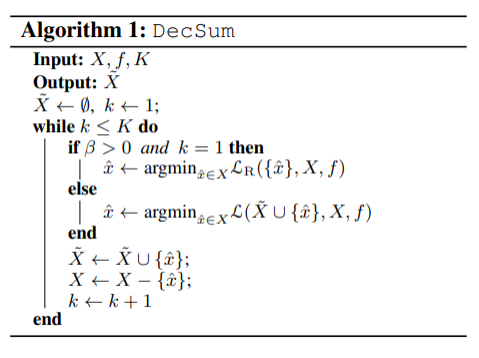
\includegraphics[scale=0.6]{../assets/DecSum_Algo}
\end{figure}

\subsection{Datasets}
%Describe the datasets you used and how you obtained them.
We used the Yelp dataset, provided freely on the \href{https://www.yelp.com/dataset/download}{\blue{Yelp website}}.

\subsection{Hyperparameters}
%Describe how you set the hyperparameters and what was the source for their value (e.g., paper, code, or your guess).
One hyperparameter group we used was what values to use for the three desiderata (decision faithfulness, decision representativeness, textual non-redundancy) when implementing DecSum.
We ran our experiments using the same as the ones given in Table 1 of their paper, as reformatted below. Note that "\textbf{Full}" in the table refers to using all the reviews without summarization,
and \textbf{MSE} is the mean-squared error.

\begin{center}
\texttt{DecSum} with ($\alpha$ decision faithfulness, $\beta$ decision representativeness, $\gamma$ textual non-redundancy)
\begin{tabular}{|c|c|c|}
    \hline
    \textbf{Method} & \textbf{MSE with Full (faithfulness)} & \textbf{MSE} \\
    \hline
    (1, 1, 1) & 0.0005 & 0.136 \\
    \hline
    (1, 1, 0) & 0.0378 & 0.164 \\
    \hline
    (1, 0, 1) & 0.0002 & 0.135 \\
    \hline
    (0, 1, 1) & 0.162  & 0.283 \\
    \hline
    (1, 0, 0) & 0.0264 & 0.155 \\
    \hline
    (0, 1, 0) & 0.175  & 0.287 \\
    \hline
    (0, 0, 1) & 0.504  & 0.565 \\
    \hline
\end{tabular}
\end{center}

\subsection{Implementation}
%Describe whether you use the existing code or write your own code, with the link to the code and which languange/packages were used. Note that the github repo you link should be public and have a clear documentation.
We use the author’s code, provided on \href{https://github.com/ChicagoHAI/decsum}{\blue{their Github}}. Python and bash shell script were used; the python packages used were
\{argparse, collections, datetime, glob, gzip, json, logging, nltk, numpy, os, pandas, pathlib, pickle, pprint, pytorch\_lightning, scipy, sentence\_transformers, sklearn, spacy, summa, time, torch,
tqdm, typing, wandb\}.

\subsection{Experimental Setup}
%Explain how you ran your experiments, e.g. the CPU/GPU resources and provide the link to your code and notebooks.
TODO

\subsection{Computational Requirements}
%Provide information on computational requirements for each of your experiments. For example, the number of CPU/GPU hours and memory requirements.
%Mention both of your estimation before running the experiments and actual resources took for reproducing the experiments.
%You'll need to think about this ahead of time, and write your code in a way that captures this information so you can later add it to this section.
The authors preprocess their data and train their model on a single RTX 3090 setup. The performance of a Tesla T4 seems to lag behind an RTX 3090, tho not overly so as one would expect from, say, a
3090 and a 1080ti, and so we expect that the GPU hours we will spend on training and processing the data to be a few hours more than that of the authors. For reference, the authors spent an hour per
epoch on fine-tuning the regression models before DecSum was ran, and less than an hour on DecSum itself. The memory requirements shouldn’t be insane, as the yelp dataset itself is only 13 GB.

\section{Results}
%Start with a high-level overview of your results. Does your work support the claims you listed in section \ref{claims}? Keep this section as factual and precise as possible, reserve your judgment and discussion points for the ``Discussion'' section that comes later.
%Go into each individual result you have, say how it relates to one of the claims and explain what your result is. Logically group related results into sections. Clearly state if you have gone beyond the original paper to run additional experiments and how they relate to the original claims.
%Tip 1: Be specific and use precise language, e.g. ``we reproduced the accuracy to within 1\% of reported value; that upholds the paper's conclusion that it performs much better than baselines.'' Getting exactly the same number is in most cases infeasible, so you'll need to use your judgment to decide if your results support the original claim of the paper.
%Tip 2: You may want to use tables and figures to demonstrate your results.
% The number of subsections for results should be the same as the number of hypotheses you are trying to verify.
TODO

\subsection{Result 1}

\subsection{Result 2}

\subsection{Additional Results not Present in the Original Paper}
%Describe any additional experiments beyond the original paper. This could include experimenting with additional datasets, exploring different methods, running more ablations, or tuning the hyperparameters. For each additional experiment, clearly describe which experiment you conducted, its result, and discussion (e.g., what is the indication of the result).
TODO

\section{Discussion}
%Describe larger implications of the experimental results, whether the original paper was reproducible, and if it wasn’t, what factors you believe made it irreproducible.
%Give your judgment on whether  the evidence you got from your experiments supports the claims of the paper. Discuss the strengths and weaknesses of your approach---perhaps you didn't have time to run all the experiments, or perhaps you did additional experiments that further strengthened the claims in the paper.
TODO

\subsection{What was Easy}
%Describe which parts of your reproduction study were easy. E.g., was it easy to run the author's code, or easy to reimplement their method based on the description in the paper. The goal of this section is to summarize to the reader which parts of the original paper they could easily apply to their problem.
%Tip: Be careful not to give sweeping generalizations. Something that is easy for you might be difficult to others. Put what was easy in context and explain why it was easy (e.g., code had extensive API documentation and a lot of examples that matched experiments in papers).
TODO

\subsection{What was Difficult}
%Describe which parts of your reproduction study were difficult or took much more time than you expected. Perhaps the data was not available and you couldn't verify some experiments, or the author's code was broken and had to be debugged first. Or, perhaps some experiments just take too much time/resources to run and you couldn't verify them. The purpose of this section is to indicate to the reader which parts of the original paper are either difficult to reuse, or require a significant amount of work and resources to verify.
%Tip: Be careful to put your discussion in context. For example, don't say ``the math was difficult to follow,'' say ``the math requires advanced knowledge of calculus to follow.''
TODO

\subsection{Recommendations for Reproducibility}
%Describe a set of recommendations to the original authors or others who work in this area for improving reproducibility.
TODO

\section*{Communication with Original Authors}
%Document the extent of (or lack of) communication with the original authors. To make sure the reproducibility report is a fair assessment of the original research we recommend getting in touch with the original authors. You can ask authors specific questions, or if you don't have any questions you can send them the full report to get their feedback.
TODO

\bibliography{projectv1}

\end{document}
